\documentclass{article}

\usepackage{fancyhdr}
\usepackage[parfill]{parskip}
\usepackage{tikz}

\pagestyle{fancyplain}

\author{Todd Davies}
\title{3.2.8 Taxonomy}
\date{\today}

\begin{document}

\rhead{3.2.8 Taxonomy}
\lhead{\today}

\maketitle

\section*{Classification}
\thispagestyle{empty}

Classification is putting organisms into groups, and giving them names suited to
their characteristics. Such organisation makes scientific work easier.

There are seven levels of taxonomic groups, and each organism belongs to one
group at each level, and so there is no overlap. The heirachy is as follows:

\marginpar{Ignore the domain group, it's not on the specification.}

\begin{center}
	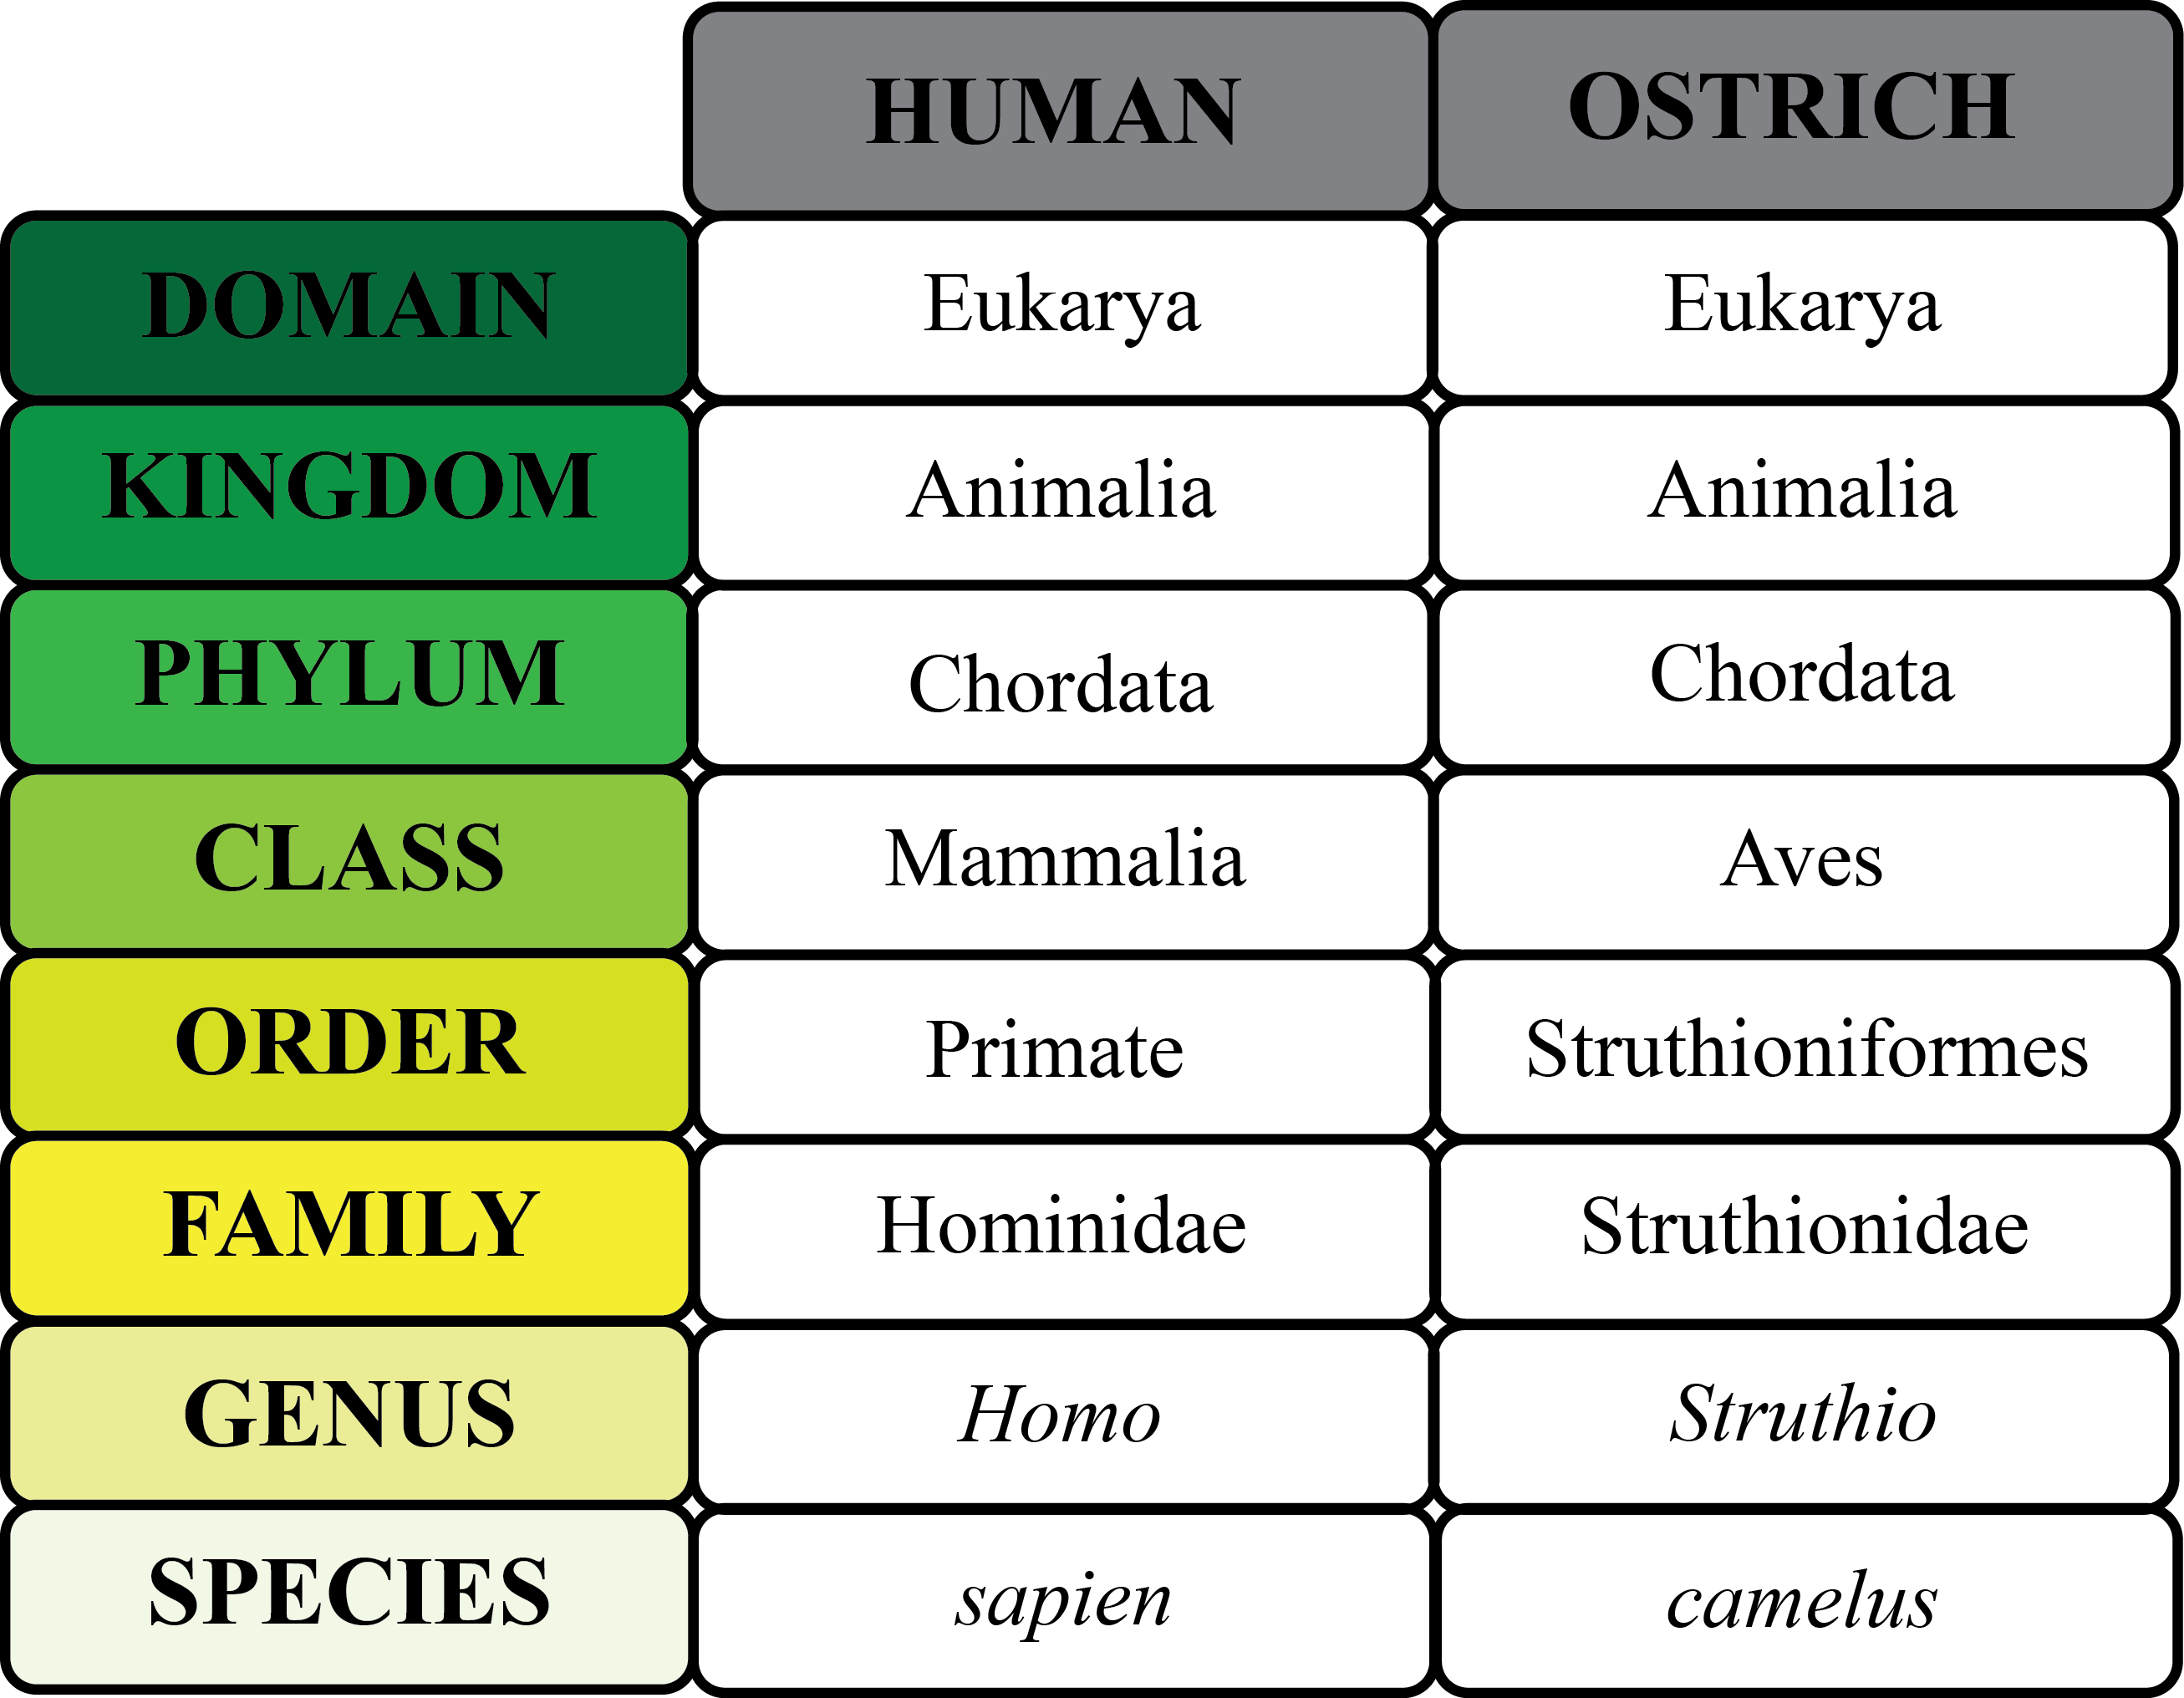
\includegraphics[scale=0.4]{taxonomic_groups}
\end{center}

As you move down the heirachy, there are more groups, but fewer organisms in
each group. Each level gets more specific.

The definition of a species is as follows:

{\it A species is a group of similar organisms able to reproduce to give fertile
offspring.}

The scienfitic name of an organism is it's genus followed by its species.

The classification systems are constantly being updated since new discoveries
about species are being made all the time.

\section*{Phylogenetics}

Phylogenetics is the study of the evolutionary history of organisms. All
organisms shared one common ancestor, but phylogenetics tells us which species
are related and how closely related they are.

Defining organisms into their proper place in the phylogenetic tree can be very
hard. Some species are extinct and so it's hard to observe their characteristics
properly, others may reproduce asexually and so it's hard to tell what parents
have had what offspring, and some similar species (e.g. humans and chimps) may
be able to produce fertile offspring, but it would be unethical to try.

It's often easier to compare the DNA of organisms, though there are no hard and
fast rules about how much DNA must differ between different species.

\end{document}